\chapter{Level 0 to 1}

The initial step in the IDEX data pipeline is to convert level 0 data to level 1. This entails two steps; namely,

\begin{enumerate}
\item \textbf{Level 0 to 1A}: Converting CCSDS packets to Time tagged event data, coincident, target and ion grid waveforms, and time-of-flight spectra in data number (DN)
\item \textbf{Level 1A to 1B}: Taking the 1A data and converting the data number spectra to voltage spectra.
\end{enumerate}

\subsection{Jamey Meeting (1/14/22)}
\begin{itemize}
    \item Python “0 to 1” code can be handed over to the SOC instead of pseudo code
\item Packetcrushing code will be useful for calibration
\item CCSDS decommutation in Python may be available
\item Make sure APID’s are in order for the CCSDS packets (FPGA testing) - reach out to Wendy \textbf{Completed that same day}
\item Get the definitions, and try to write it with the synthetic spectra and test it
\item 1: dN, 2: Volts, 3: ion mass
\item Make sure we interface with the mapping groups (ENA pipeline is not so different than our instrument)
\end{itemize}


The contents of each APID are further described below.  All IDEX packets are \textbf{32-bit aligned, start with a CCSDS header, and end with a 2-byte CRC} (see IICD JPL D-55881 for details).  A 32-bit Unified Message Structure header appears before the CCSDS header, but is expected to be removed by the spacecraft before it get to the ground.
\newline
\newline
In general, science data is organized onboard by the \textbf{accountability identifier (AID)}.  The AID is assigned when the data is acquired, and is used to access the data afterwards.  The AID cannot be changed, and duplicate AIDs are not permitted.  Each dataset is composed of one or more \textbf{“events”}, which is a collection of data collected when the instrument triggers, usually representing a dust particle impact.  Each event is given a unique “event number” by the FPGA, so that every event collected by IDEX can be uniquely identified by the combination of AID and event number.  

SUDA Event data is composed of seven distinct parts:
\begin{enumerate}
\item	Time of Flight (TOF) waveform data on the high-gain (HG) channel, sampled at 250 megasamples per second (Msps) with 10 bit resolution
\item	TOF waveform data on the mid-gain (MG) channel, sampled at 250 Msps with 10 bit resolution
\item	TOF waveform data on the low-gain (LG) channel, sampled at 250 Msps with 10 bit resolution
\item	Velocity (Qv) grid charge sensitive amplifier (CSA) waveform data, sampled at 3.75 Msps with 12 bit resolution
\item	Ion (Qi) grid CSA waveform data, sampled at 3.75 Msps with 12 bit resolution
\item	Target (Qt) CSA waveform data, sampled at 3.75 Msps with 12 bit resolution
\item	FPGA Pre-pended metadata header containing IDEX’s configuration and status at the time of the trigger, recorded by the FPGA
\end{enumerate}


\section{Heritage Processing}
This section describes the development of Python code to convert level 0 data to level 1A. The code described below can be found in the pipeline dropbox under "/python/Level 0$\rightarrow$1/Python Packet Crushing"

\begin{figure}[H]
    \centering
    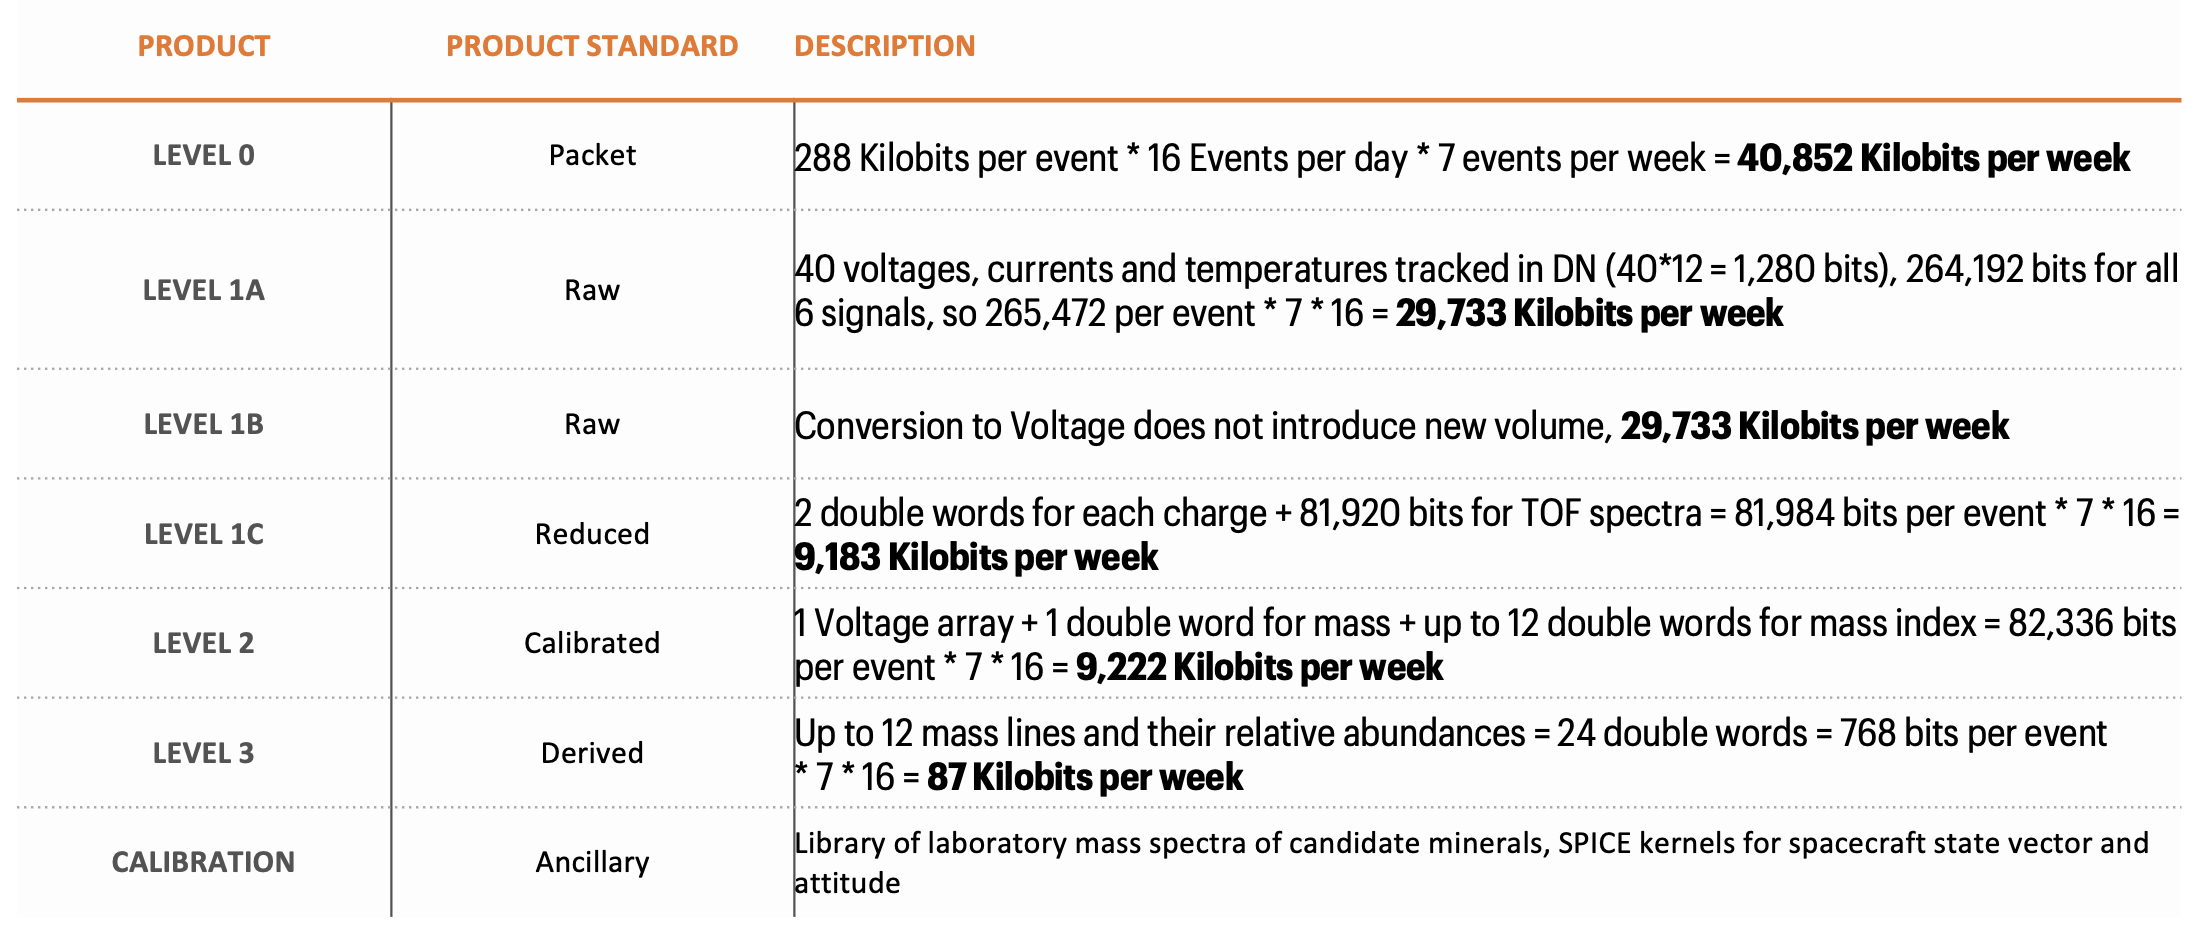
\includegraphics[width=\linewidth]{images/DataVolume.png}
    \caption{An outline of the data volume by product level. This is based on FPGA buffers and packetizing overhead.}
    \label{fig:datavolume}
\end{figure}

\begin{figure}[H]
    \centering
    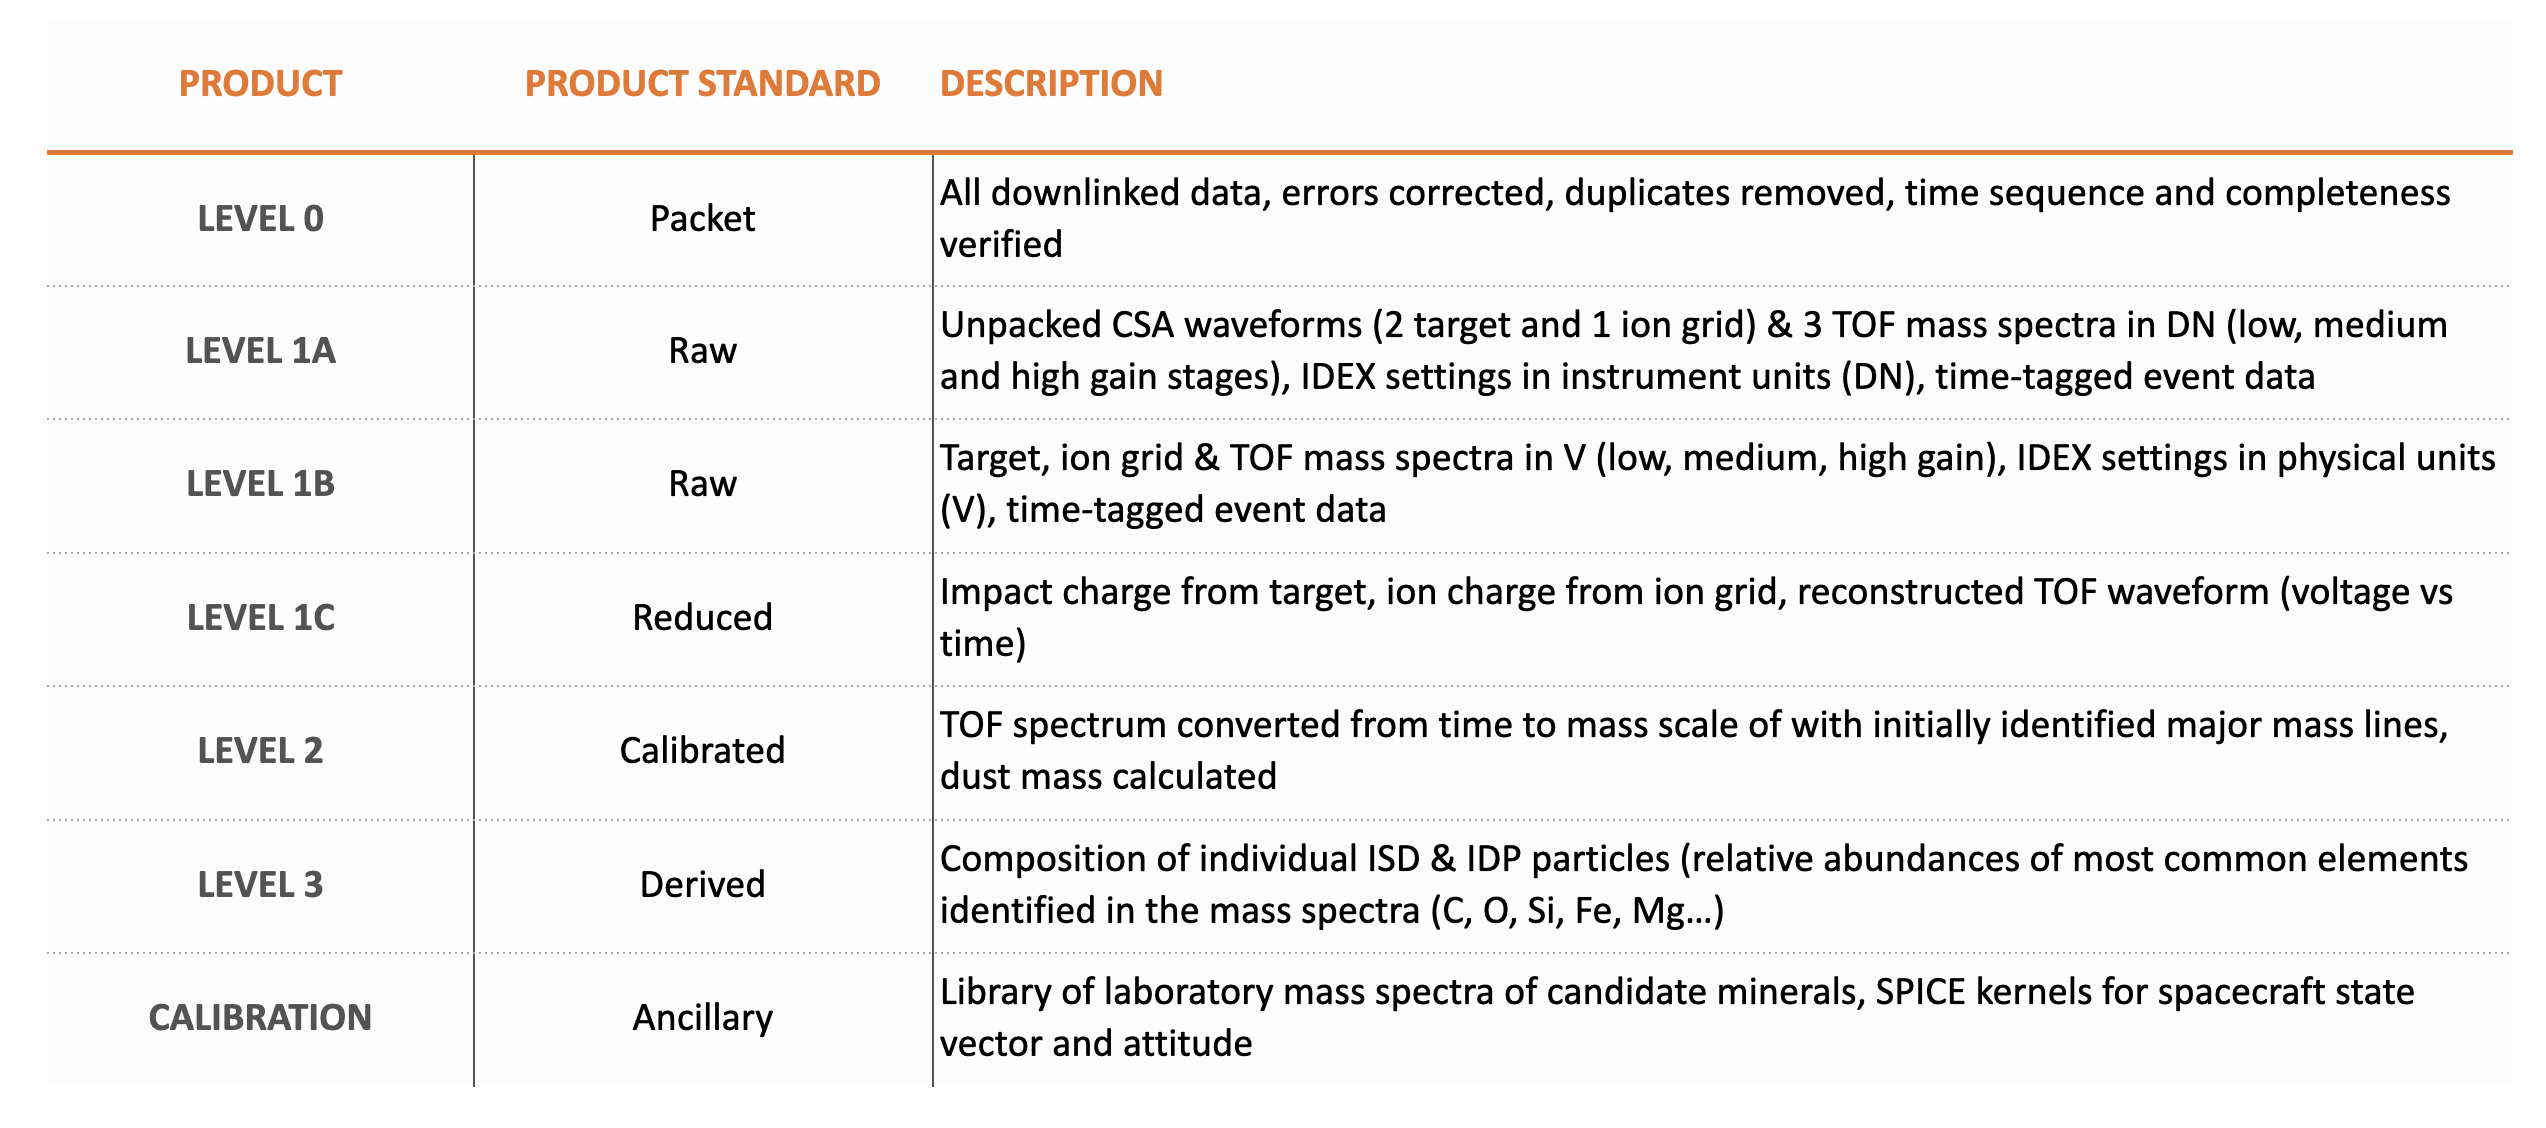
\includegraphics[width=\linewidth]{images/pipeline.png}
    \caption{An outline of each data product level containing the corresponding data type and description.}
    \label{fig:pipeline}
\end{figure}





\begin{figure}[H]
    \centering
    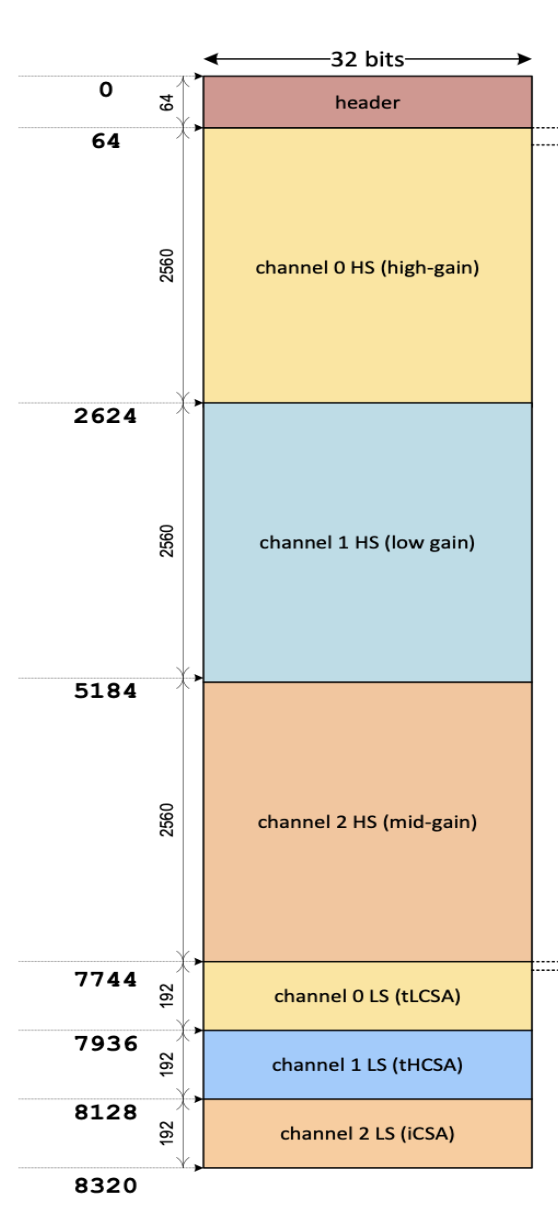
\includegraphics[width=\linewidth]{images/Waveform_Structure.png}
    \caption{An outline of IDEX's channels, with their bit length. Only specific packets contain waveforms.}
    \label{fig:db}
\end{figure}
\subsection{Hydra Packets:}
We chose to start by reading in the Hydra science packets from their raw .xml files. These files are similar to html, minus the prewritten tags. They follow the anatomy delineated in the figure below:


\begin{figure}[H]
    \centering
    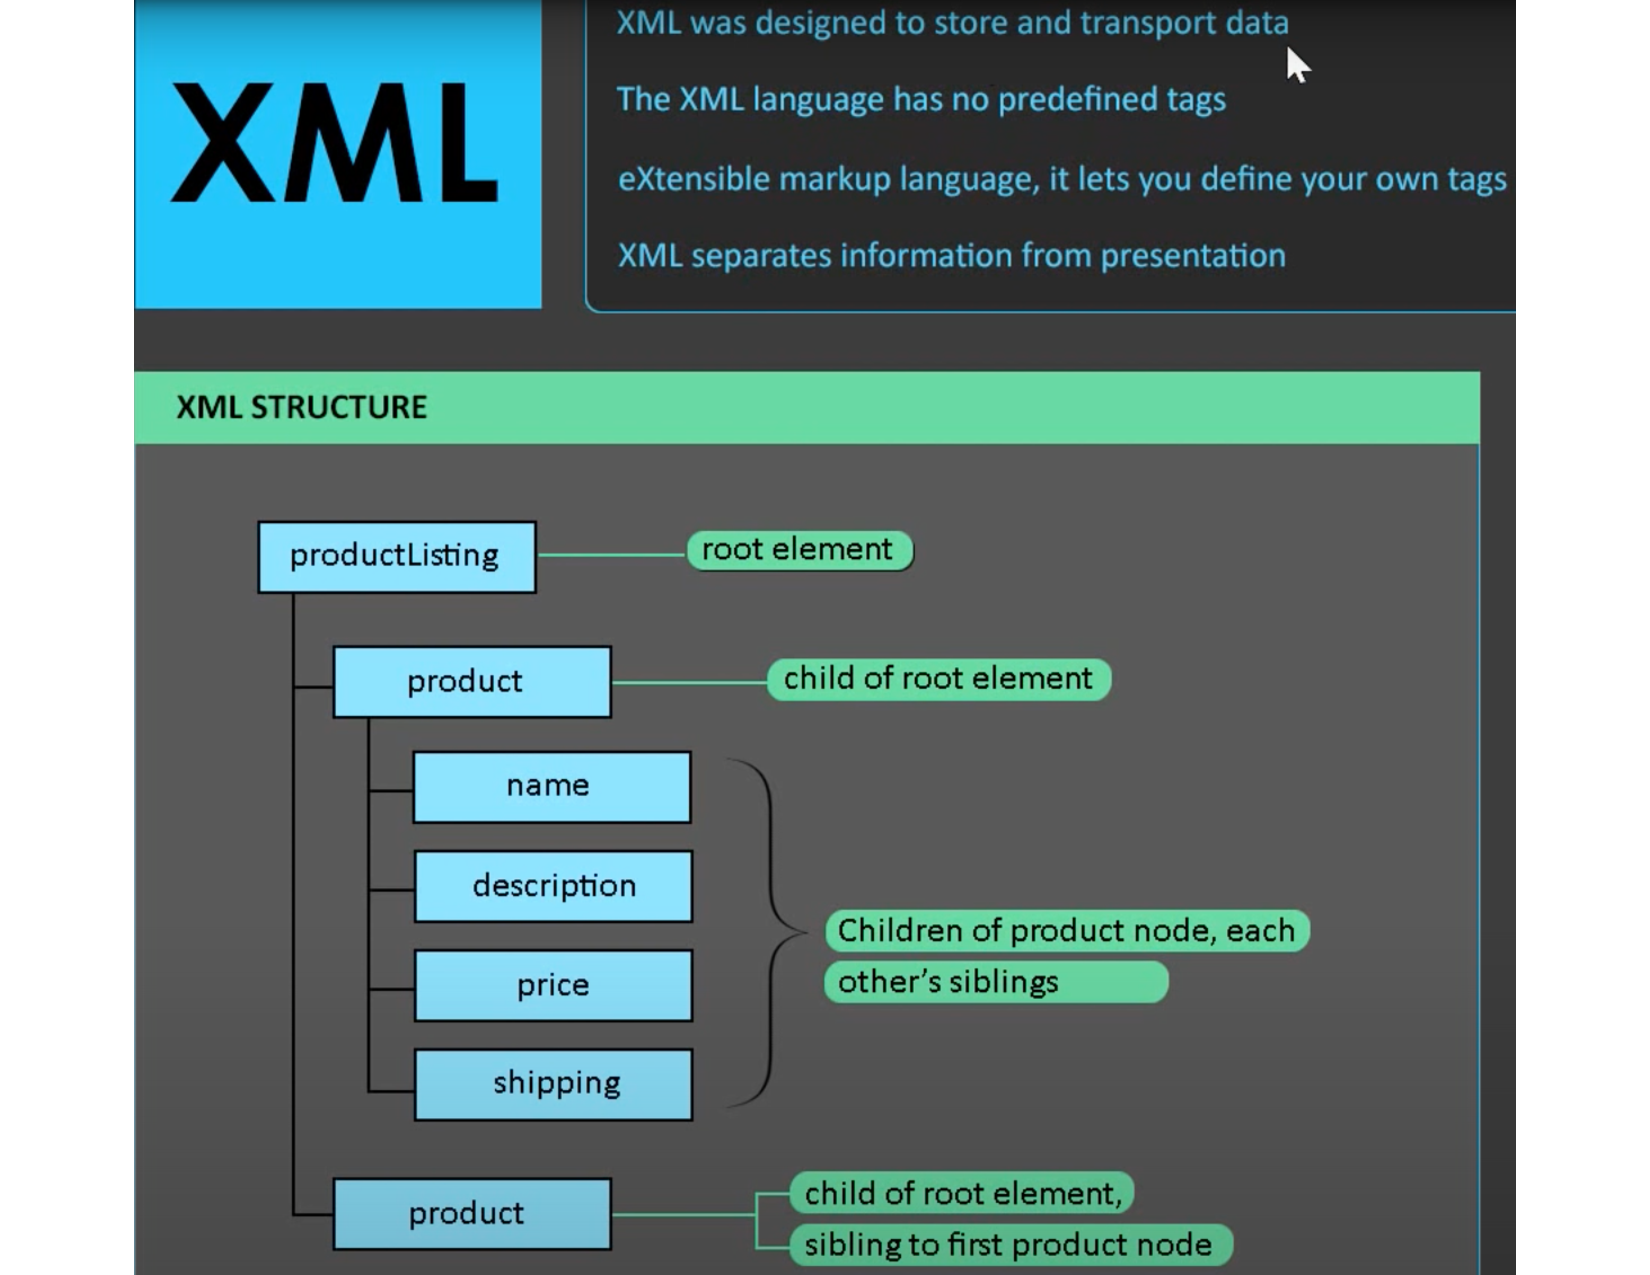
\includegraphics[width=12cm]{images/xml.pdf}
    \caption{Anatomy of an xml document along with some general notes. }
    \label{fig:massline-byloc}
\end{figure}


\section{Next steps:}
\begin{enumerate}
\item Focus on ion calibration part of the packet
\item Once we get level 0, the TOF channel is this large with this many units, etc. $\rightarrow$ Data volume figure \ref{fig:datavolume}
\item Give dtypes and volumes from SDC document $\rightarrow$ White paper
\item Describe the APIDS we've inherited from SUDA $\rightarrow$ Outlined, finish translating white paper
\item Describe hierarchical decision tree $\rightarrow$ Text description from greg, make a diagram
\item Provide the calibration curve in terms of the fits (The final calibration) $\rightarrow$ Heritage SUDA and LDEX curves available

\end{enumerate}
